\documentclass[tikz,border=6pt]{standalone}
\usepackage{xcolor}
\usetikzlibrary{arrows.meta,decorations.pathmorphing,calc,positioning,fit,backgrounds,shapes.geometric}
\definecolor{red}{HTML}{A50F2D}\definecolor{ink}{HTML}{141414}\definecolor{gry}{HTML}{5F5F5F}\definecolor{lgry}{HTML}{E6E6E6}
\definecolor{blu}{HTML}{2B6CB0}\definecolor{teal}{HTML}{1B9E8F}\definecolor{org}{HTML}{E8702A}\definecolor{grn}{HTML}{2E9E5B}\definecolor{mag}{HTML}{D81B60}\definecolor{pur}{HTML}{5B2C83}
\tikzset{fibre/.style={ink,line width=1.6pt,line cap=round},
 sis1/.style={org,line width=1.8pt,line cap=round},sis2/.style={blu,line width=1.8pt,line cap=round},
 lab/.style={font=\sffamily\small,text=ink},lbl/.style={font=\sffamily\footnotesize,text=gry,align=center},ttl/.style={font=\sffamily\bfseries\small,text=ink},
 ctcf/.style={-{Triangle[length=5pt,width=6pt]},pur,line width=2.4pt},
 cohesin/.style={grn,line width=1.6pt}}

% ---- shared drawing macros: a DNA duplex is a dark tube with a light core
\newcommand{\dx}[2][ink]{\draw[line width=3.6pt,#1,line cap=round] #2; \draw[line width=1.3pt,white,line cap=round] #2;}
% omega-shaped loop: base at (x,y), radius r
\newcommand{\omegapath}[3]{(#1-0.35,#2) .. controls (#1-0.35,#2+0.45) and (#1-#3,#2+0.35) .. (#1-#3,#2+#3+0.45) arc[start angle=180,end angle=0,radius=#3] .. controls (#1+#3,#2+0.35) and (#1+0.35,#2+0.45) .. (#1+0.35,#2)}
% replication eye: origin at (x,y), half width w, half height h
\newcommand{\eyetop}[4]{(#1-#3,#2) .. controls (#1-#3*0.5,#2+#4*1.33) and (#1+#3*0.5,#2+#4*1.33) .. (#1+#3,#2)}
\newcommand{\eyebot}[4]{(#1-#3,#2) .. controls (#1-#3*0.5,#2-#4*1.33) and (#1+#3*0.5,#2-#4*1.33) .. (#1+#3,#2)}
\newcommand{\eye}[4]{\dx[org]{\eyetop{#1}{#2}{#3}{#4}}\dx[blu]{\eyebot{#1}{#2}{#3}{#4}}\fill[teal] (#1-#3,#2) circle (3.2pt) (#1+#3,#2) circle (3.2pt);}
\newcommand{\ring}[3]{\draw[grn,line width=1.8pt] (#1,#2) ellipse (#3 and #3*1.35);}
\newcommand{\gseg}[3]{\dx[gry]{(#2,#1) -- (#3,#1)}}

\begin{document}
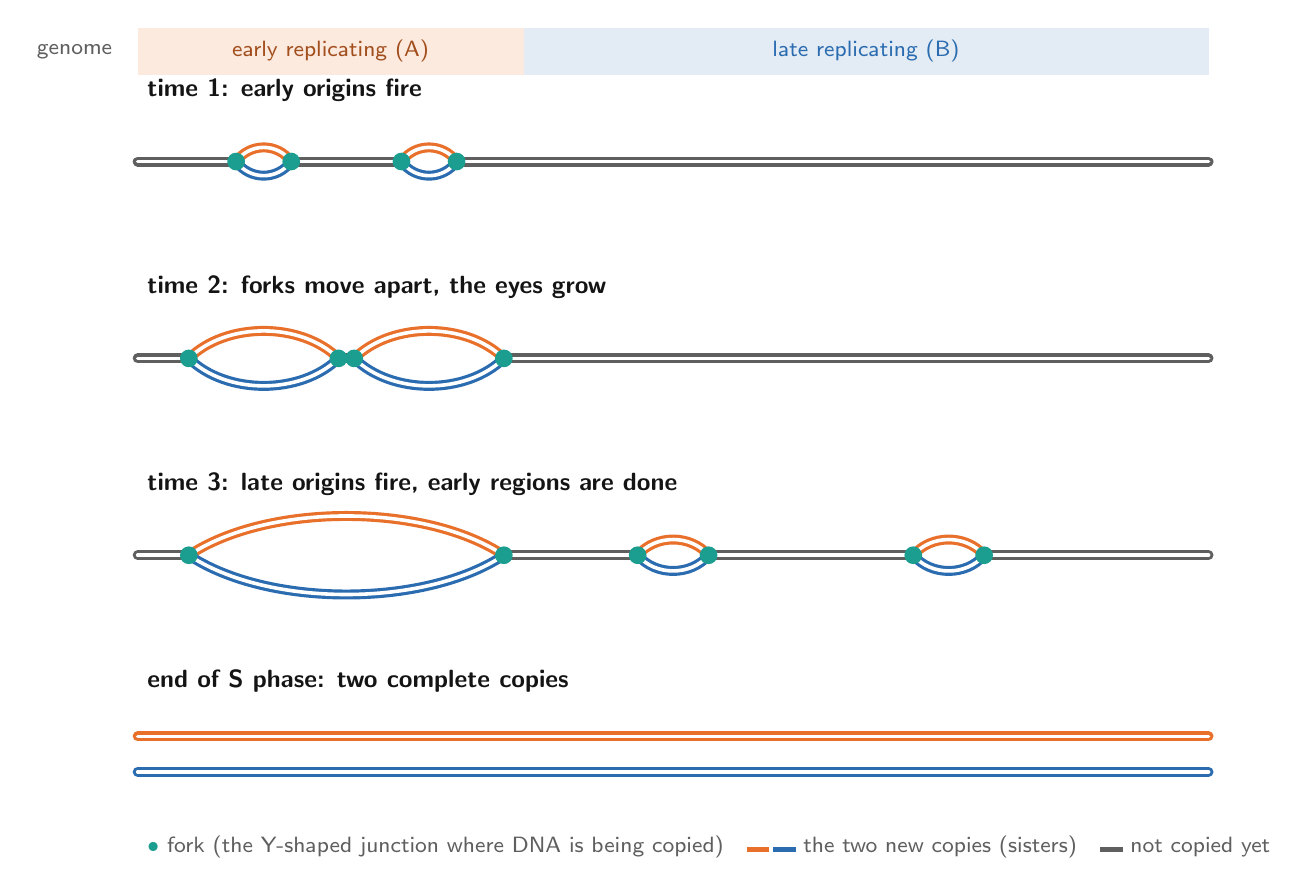
\begin{tikzpicture}[font=\sffamily\small,>=Stealth]
\fill[org!15] (-0.3,0.9) rectangle (4.6,1.5); \fill[blu!13] (4.6,0.9) rectangle (13.3,1.5);
\node[lbl,org!70!black] at (2.15,1.2) {early replicating (A)}; \node[lbl,blu] at (8.95,1.2) {late replicating (B)};
\node[lbl,anchor=east] at (-0.5,1.2) {genome};
\foreach \y/\t in {-0.2/{time 1: early origins fire},-2.7/{time 2: forks move apart, the eyes grow},-5.2/{time 3: late origins fire, early regions are done},-7.7/{end of S phase: two complete copies}}{
 \node[ttl,anchor=west] at (-0.3,\y+0.9) {\t};}
% time 1
\gseg{-0.2}{-0.3}{0.95}\gseg{-0.2}{1.65}{3.05}\gseg{-0.2}{3.75}{13.3}
\foreach \x in {1.3,3.4}{\eye{\x}{-0.2}{0.35}{0.18}}
% time 2
\gseg{-2.7}{-0.3}{0.35}\gseg{-2.7}{2.25}{2.45}\gseg{-2.7}{4.35}{13.3}
\foreach \x in {1.3,3.4}{\eye{\x}{-2.7}{0.95}{0.35}}
% time 3
\gseg{-5.2}{-0.3}{0.35}\gseg{-5.2}{4.35}{6.05}\gseg{-5.2}{6.95}{9.55}\gseg{-5.2}{10.45}{13.3}
\eye{2.35}{-5.2}{2.0}{0.5}
\foreach \x in {6.5,10.0}{\eye{\x}{-5.2}{0.45}{0.2}}
% end
\dx[org]{(-0.3,-7.5) -- (13.3,-7.5)} \dx[blu]{(-0.3,-7.95) -- (13.3,-7.95)}
\node[lbl,anchor=west] at (-0.3,-8.9) {\textcolor{teal}{$\bullet$} fork (the Y-shaped junction where DNA is being copied)\quad \textcolor{org}{\rule{8pt}{2pt}}\,\textcolor{blu}{\rule{8pt}{2pt}} the two new copies (sisters)\quad \textcolor{gry}{\rule{8pt}{2pt}} not copied yet};
\end{tikzpicture}
\end{document}
